\subsection{Arg Max}
Arg Max, or arguments of the maxima, are the inputs at which a function or sequence takes on a maximum value.  It can be seen as a special case of max pooling where the pool size and stride are equal to the length of the signal of interest.  In our implementation of the neural net architecture, we deviated here.  The architecture includes what is called a `Softmax' (which is short for soft arg max) function at the very end of the neural net which maps the output of the previous stage to a vector of elements in $(0,1)^{10}$ which represents the neural net's `confidence' about a given modulation scheme.  This is done using sums and quotients of exponential functions, which are very numerically unstable, especially for fixed point.  We chose to do away with this stage and instead replace it with an arg max.  Since softmax preserves ordering, a simple arg max will result in the same decision being made, it doesn't hurt performance at all.  Currently the design and implementation is a farily naive combinational one which was automatically generated by Vivado.  However, the output has been tested and correctly gives the maximum input.  A sample result is shown in figure \ref{fig:argmax}

\begin{figure}[H]
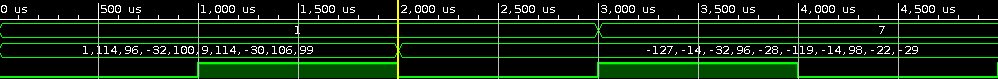
\includegraphics[width=\textwidth]{argmax.png}
\caption{Example output of arg max}
\label{fig:argmax}
\centering
\end{figure}
